%intro to sequence analysis
Magnitude analysis and categorization are both appropriate for answering research questions that are simply manifested in the IDE usage log. However, a more powerful way of analyzing activity logs is through sequence analysis, which first breaks the IDE data stream into a number of sequences, according to some criteria, and then reports upon characteristics of each sequence. A sequence in the IDE usage data corresponds to a software engineering task or sub-task accomplished by the user (e.g. refactoring, looking for a starting point for a maintenance task, etc.), consisting of all of IDE events in a given time span. For instance, answering the research question of ``Are developers successful at finding initial points in the code for a software maintenance task?'' requires that the sequence of IDE events corresponding to each maintenance task be identified, before we can perform further analysis using either magnitude or categorization analysis. The granularity of a sequence is determined by the guiding research question. For certain research questions, we may be interested in a smaller sequences (e.g. searching the code base), while for others we may need to consider a longer time span (e.g. implementing a new feature, fixing a bug). 
Generally, the larger and more complex the task or sub-task to extract, the harder it is for sequence analysis to determine its starting and stopping point in the activity log~\cite{Zou-ComanIndustry}.

%how difficult or easy is it to determine sequences
In many cases, extracting activity sequences can be challenging as it impossible to know exactly when a developer begins or ends a particular task or sub-task, without understanding the developer's underlying thought process. There are several possibilities in how sequence extraction can be performed, based on the specific research question. One possibility is to use sentinels, which are specific actions that indicate the beginning and end of a sequence. For instance, in the context of the code search research question mentioned above, submitting a query to the code search tool begins a sequence, while performing an edit or structural navigation (e.g. following the call graph) ends the sequence. Another possibility is to use the passage of time to extract sequences, where time without any activity is used as a signal of task start or finish. Yet another possibility is to use locations in the code base to identify a sequence in the activity log. This is the key insight used in Coman et al.'s \cite{Coman-TaskIdent} algorithm, which uses periods of activity on the same program elements to represent the core of a task, and time distance between such events to extract sequences corresponding to developer tasks. In lab validation studies of this algorithm have shown very high accuracy (80\%) when compared to the ground truth reported by developers. However, this accuracy may not hold up in an industrial setting\cite{Zou-ComanIndustry}, where tasks are longer, code bases are more complex, and developer interruptions are common. Also, the algorithm requires that information regarding program elements is kept in the activity log, which may conflict with many developer's privacy and anonymity requirements.

%example
We illustrate sequence analysis given the research question  ``Are developers successful at finding initial points in the code for a software maintenance task?'' and the following usage log.

\begin{verbatim}
Collector Started
2014-02-02 13:46:52 - User submitted query to Find-in-Files
2014-02-02 13:46:56 - Find-in-Files retreived 121 results
2014-02-02 13:52:21 - User clicked on result 2
2014-02-02 13:58:01 - User clicked on result 8
2014-02-02 13:59:57 - Open caller/callee command 
...
2014-02-02 14:46:52 - User submitted query to Find-in-Files
2014-02-02 14:46:56 - Find-in-Files retreived 19 results
2014-02-02 15:01:08 - User clicked on result 11
2014-02-02 17:30:12 - User editted code
...
\end{verbatim}

To answer the research question, sequence analysis can extract two separate sequences in the above log by using sentinels indicative of start/end of a code search activity, among other possible sequence identification approaches. Both of the extracted search sequences can be deemed as successful since for each of the queries to the {\tt Find-in-Files} code search tool the user clicks on a retreived result, followed by a structured navigation event (open caller/callee) or editing event (user edited code). Therefore it would seem that the developer is successful at finding initial points in the code for his or her software maintenance task. However, on closer inspection of the second sequence, we observe that there is a large time gap between clicking on a result and editing code. The reason for this time gap is open to interpretation, as the developer may have returned to the previous results, continuing the search session, or have started on a completely new development activity. Certain types of sequence analysis, such as Coman's algorithm, take time into account when identifying sequences, while others, like the sentinel approach used above, do not. Neither of these approaches, however, helps to resolve the origin of ambiguous events, which are left to the researcher to characterize.

%\begin{figure*}[t]
%\centering
%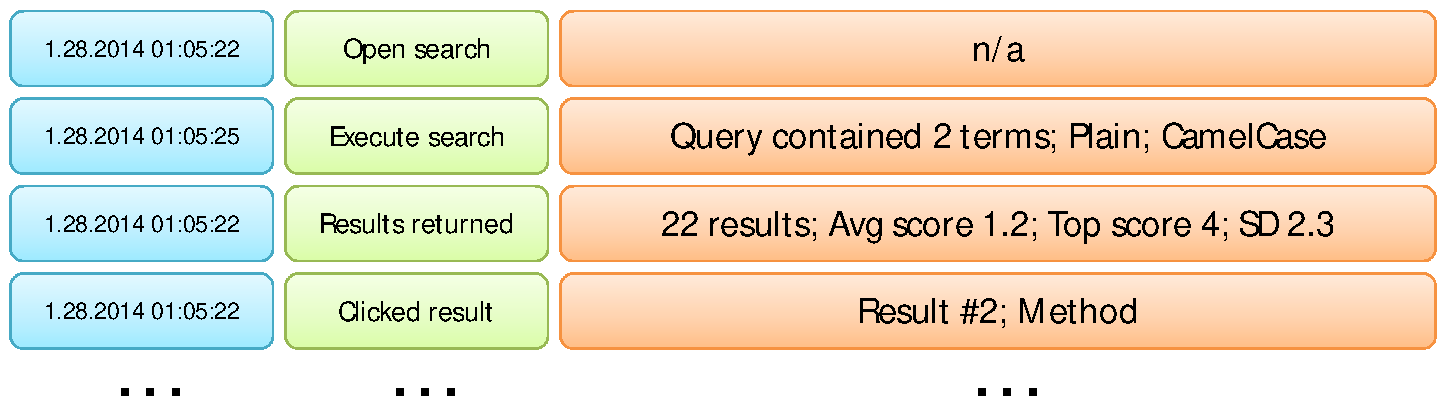
\includegraphics[width=1\columnwidth]{../Graphics/activityLogActual.pdf}
%\caption{Pairwise matches across categories, including matching and mismatching pairs.}
%\label{fig:actual}
%\end{figure*}



